\chapter{Results} \label{results}
%\begin{figure}[H]
%\centering
%    \begin{minipage}{0.45\textwidth}
%%        \centering
%        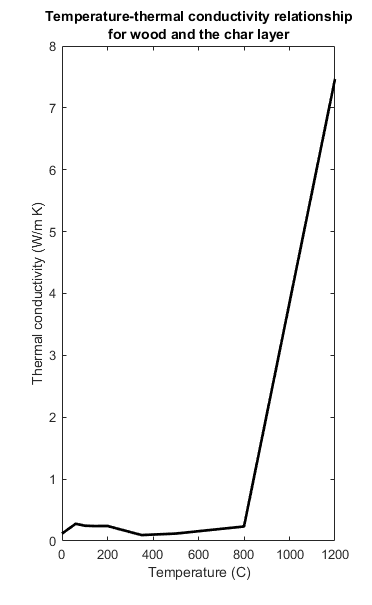
\includegraphics[width=0.9\textwidth]{figures/resultsk_cropped.png} % first figure itself
%        \caption{The resulting $\kappa$-values }
%        \label{kresult_fig}
%    \end{minipage}
%    \begin{minipage}{0.45\textwidth}
%%        \centering
%        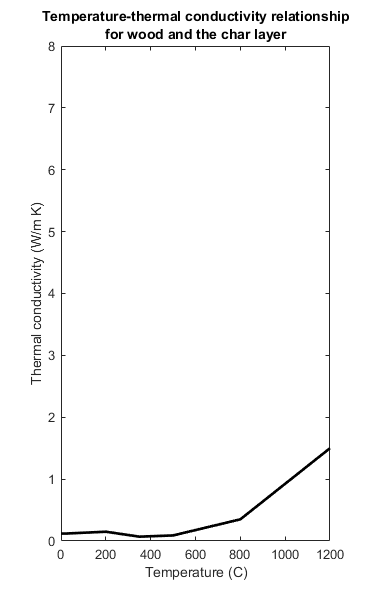
\includegraphics[width=0.9\textwidth]{figures/eurok_samescale_cropped.png} % second figure itself
%        \caption{The original $\kappa$-values}
%        \label{scalekeuro_fig}
%    \end{minipage}
%\end{figure}\

The results of running the algorithm until 20 000 acceptable values are found is shown below.)TODO add more.
\section{Resulting k-values}

The thermal conductivity ($\kappa$-values) at key temperatures was the main goal of this project. 
As can be seen in Figure \ref{kresult_euro_fig} there was quite a drastic difference in the thermal diffusivity at 1200 \textdegree C and between 0\textdegree C and 200\textdegree C.
thee large difference at 1200\textdegree C is due to how our model is created.(TODO?)
Most of the energy at that temperature is radiated?(TODO)
\begin{figure}[H]
	\label{kresult_euro_fig}
	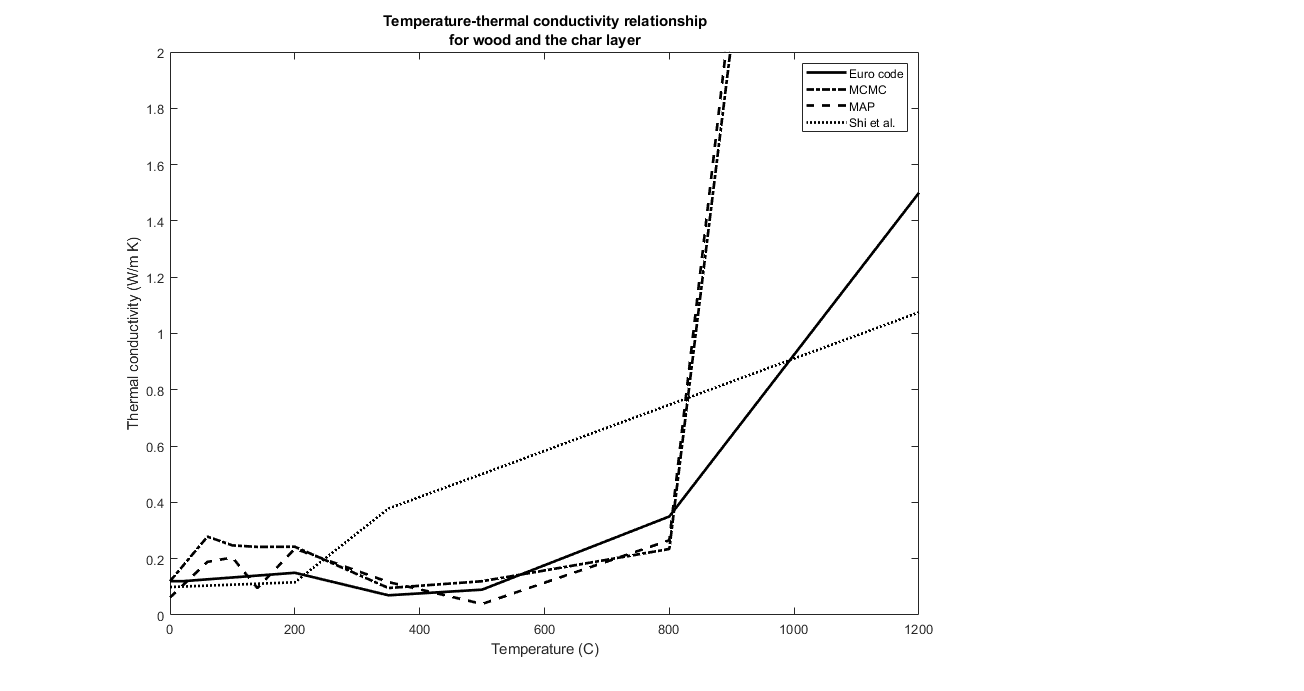
\includegraphics[width=\linewidth]{figures/kvalues_all_shi.png}
	\caption{Resulting $\kappa$ values compared to Euro-code standard values}
\end{figure}
 
\begin{figure}[b]
\label{histofig}
\centering
	\begin{subfigure}{}
	\centering
	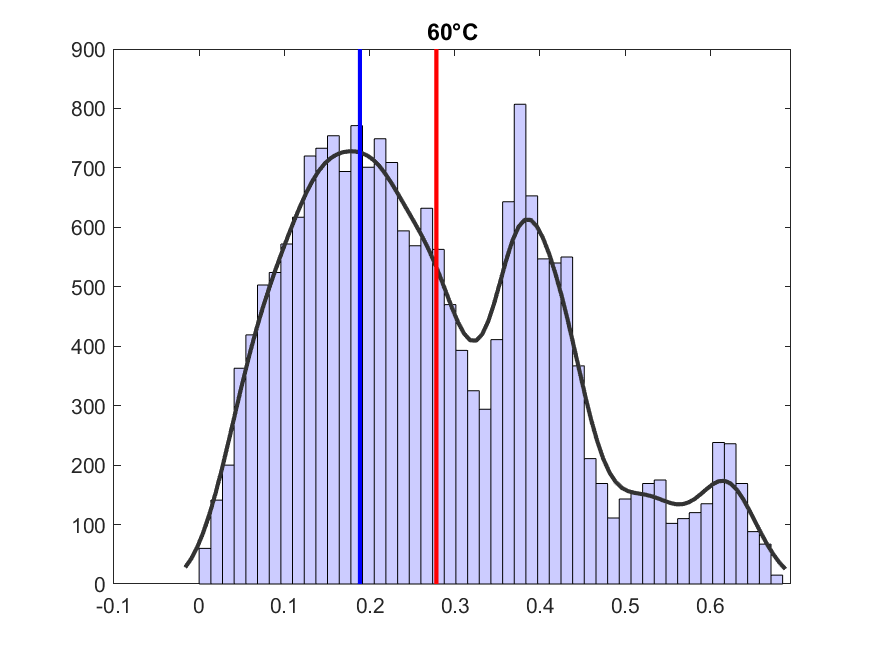
\includegraphics[width = 0.45\linewidth]{figures/histograph/histo1.png}
	\end{subfigure}
	\begin{subfigure}{}
	\centering
	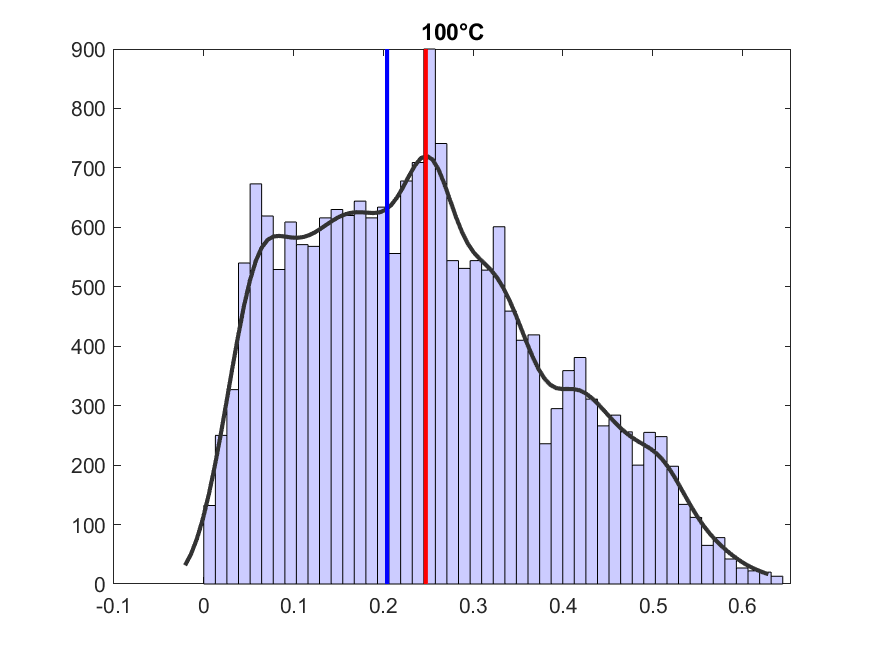
\includegraphics[width = 0.45\linewidth]{figures/histograph/histo2.png}
	\end{subfigure}
	\begin{subfigure}{}
	\centering
	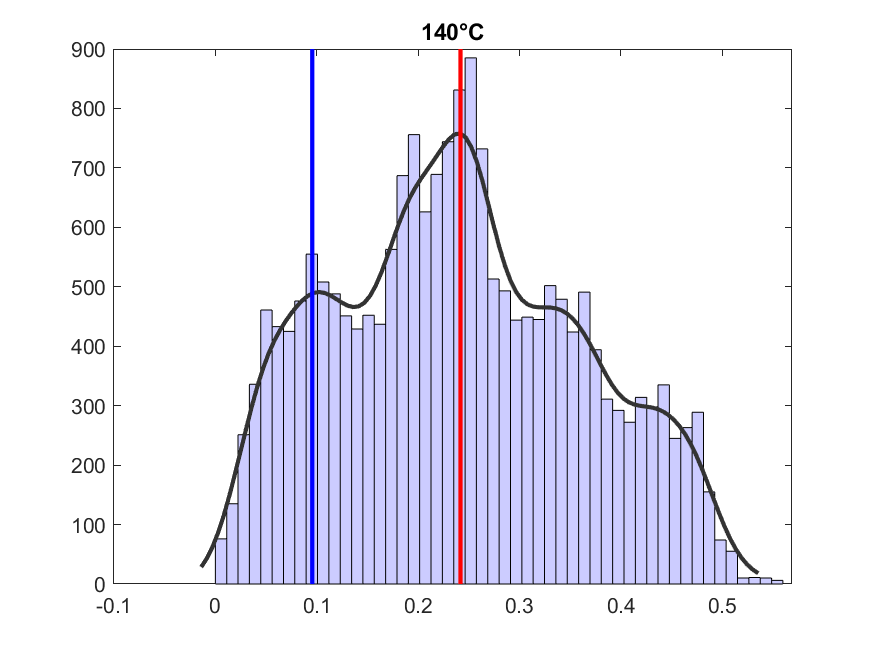
\includegraphics[width = 0.45\linewidth]{figures/histograph/histo3.png}
	\end{subfigure}
	\begin{subfigure}{}
	\centering
	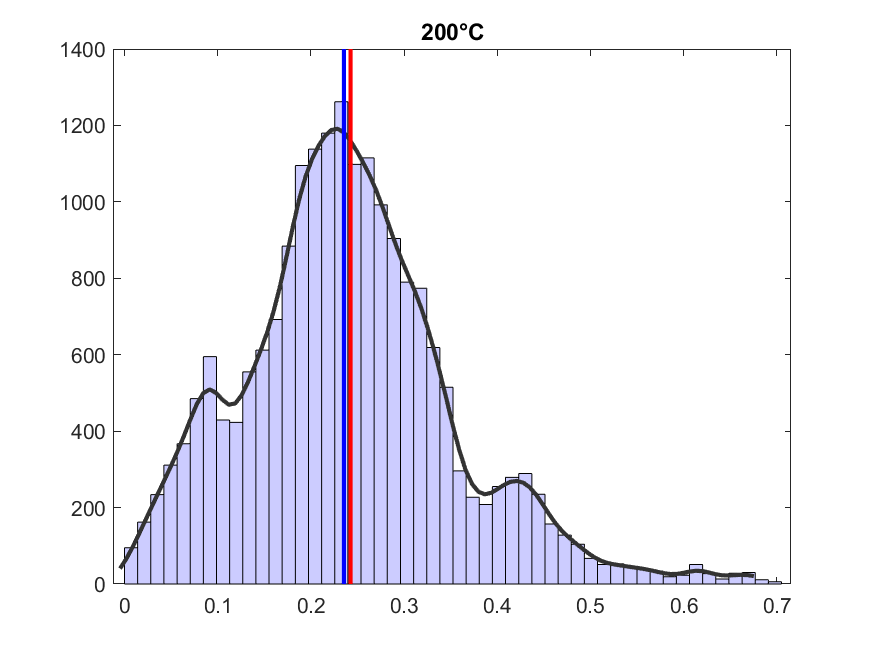
\includegraphics[width = 0.45\linewidth]{figures/histograph/histo4.png}
	\end{subfigure}
	\begin{subfigure}{}
	\centering
	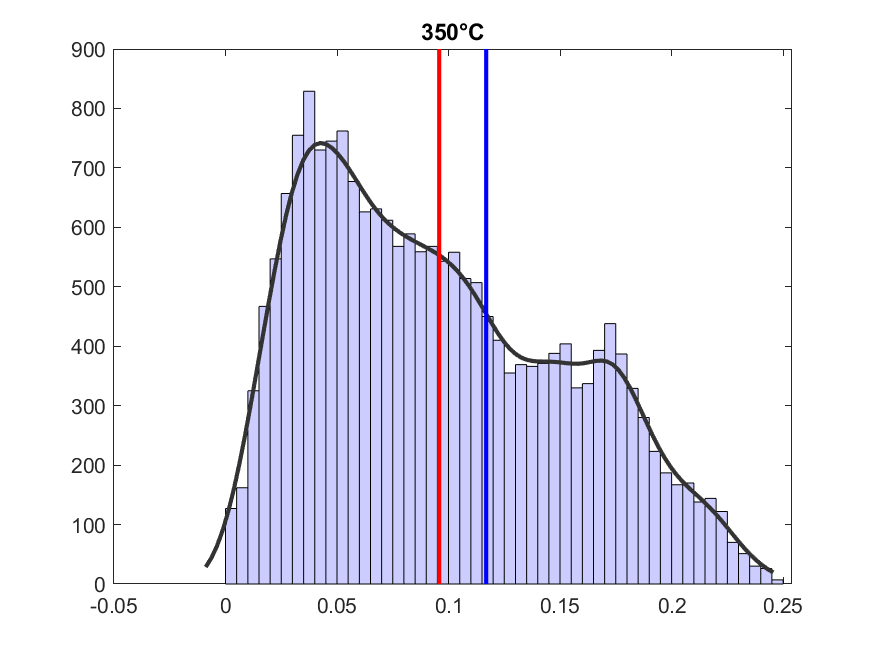
\includegraphics[width = 0.45\linewidth]{figures/histograph/histo5.png}
	\end{subfigure}
	\begin{subfigure}{}
	\centering
	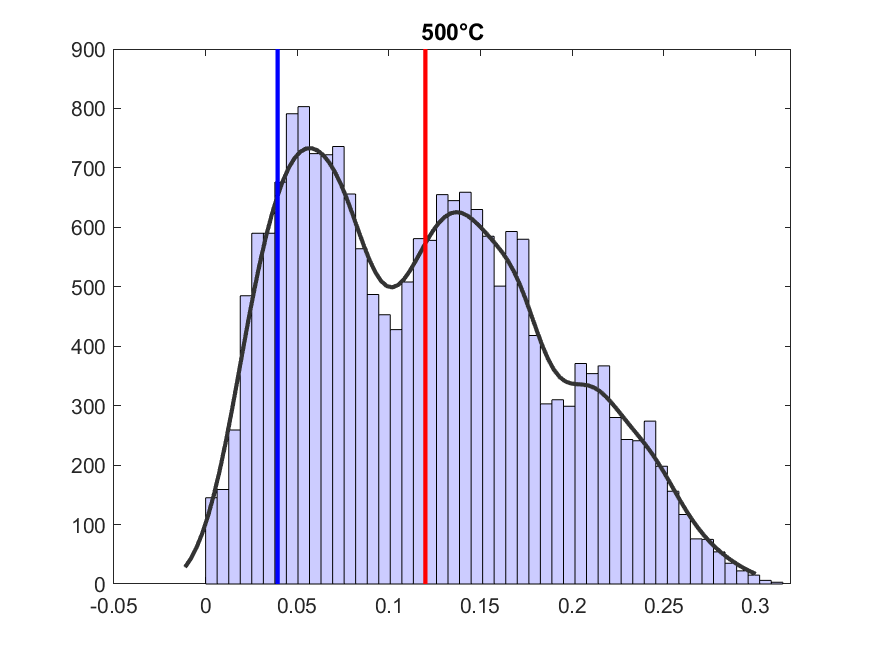
\includegraphics[width = 0.45\linewidth]{figures/histograph/histo6.png}
	\end{subfigure}
	\begin{subfigure}{}
	\centering
	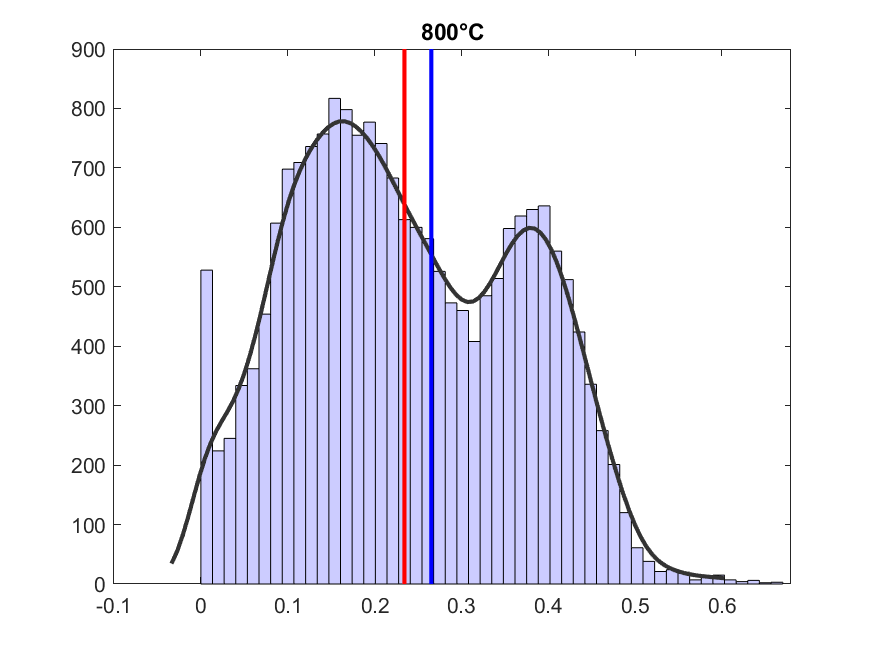
\includegraphics[width = 0.45\linewidth]{figures/histograph/histo7.png}
	\end{subfigure}
	\begin{subfigure}{}
	\centering
	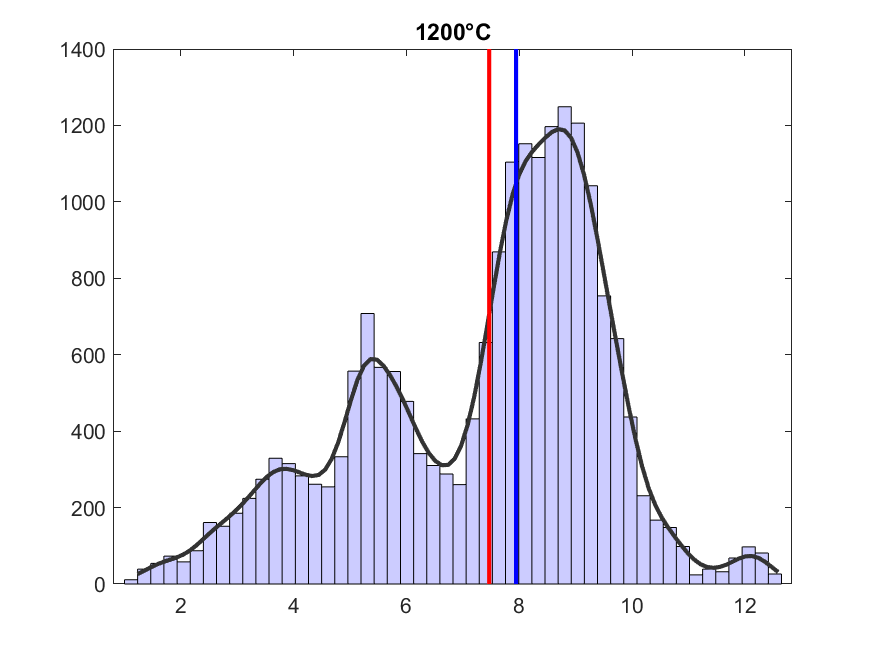
\includegraphics[width = 0.45\linewidth]{figures/histograph/histo8.png}
	\end{subfigure}
	\caption[short]{Histographs showing distribution at different temperatures}
\end{figure}


